\documentclass{beamer}

\usepackage{pres}

\title{\trtitle \\ \vspace{5pt} \footnotesize \trtype}
\author{\trauthor \\ \vspace{5pt} \footnotesize \trfach}
\date{28 April, 2015}

\begin{document}

\frame{\titlepage}

\frame{
  \frametitle{Outline}
  \tableofcontents
}

\section{Introduction}
\begin{frame}
  \frametitle{Motivation}

  \begin{itemize}
    \item Human use multiple sensory information to recognize objects.

      ~
    \item Difficulties of visual object recognition:
      \begin{itemize}
        \item Sensitive to image transformations. 
      \end{itemize}

      ~
    \item Sound provides complementary information.
      \begin{itemize}
        \item Make sound via interactions.
        \item Information about material. 
        \item Category by function: objects that make sound.
      \end{itemize}
  \end{itemize}
\end{frame}

\begin{frame}
  \frametitle{Related Work}

  \begin{itemize}
    \item Sinapov and his colleagues~\cite{sinapov_interactive_2009,sinapov_object_2011}: 
      \begin{itemize}
        \item Audio and haptic information.
        \item Relational learning.

          ~
        \item No visual information.
      \end{itemize}

      ~
    \item Nakamura and his colleagues~\cite{nakamura_multimodal_2007,nakamura_bag_2012}:
      \begin{itemize}
        \item Visual, audio and haptic information.
        \item Multimodal pLSA.

          ~
        \item Unsupervised categorization.
      \end{itemize}
  \end{itemize}
\end{frame}

\begin{frame}
  \frametitle{Objective}

  \begin{itemize}
    \item Build a object recognition system based on visual and audio information.

      ~
      \begin{itemize}
        \item What kind of features?

          ~
        \item How to make classification?

          ~
        \item How to combine multimodal information?
      \end{itemize}
  \end{itemize}
\end{frame}

\begin{frame}
  \frametitle{Two Tasks of Object Recognition}

  \begin{itemize}
    \item Specific object recognition.
      \begin{tabular}{cccc|c}
        \multicolumn{4}{c}{Train} & Test \\
        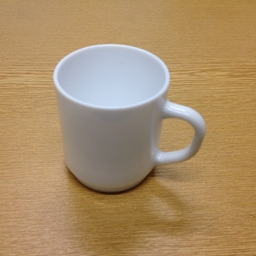
\includegraphics[width=.14\textwidth]{mug1} & 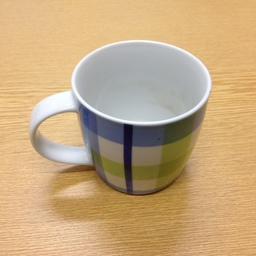
\includegraphics[width=.14\textwidth]{mug2} & 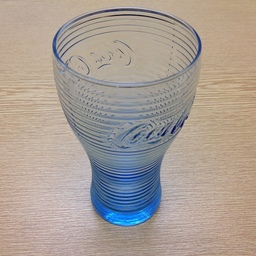
\includegraphics[width=.14\textwidth]{glass1} & 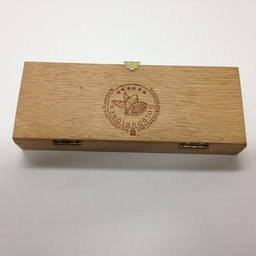
\includegraphics[width=.14\textwidth]{box1} & 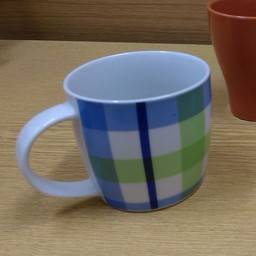
\includegraphics[width=.14\textwidth]{mug2v2} \\
        mug \#1 & mug \#2 & glass \#1 & box \#1 & mug \#2 \\
      \end{tabular}

      ~
    \item Generic category recognition.
      \begin{tabular}{cccc|c}
        \multicolumn{4}{c}{Train} & Test \\
        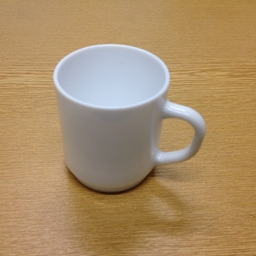
\includegraphics[width=.14\textwidth]{mug1} & 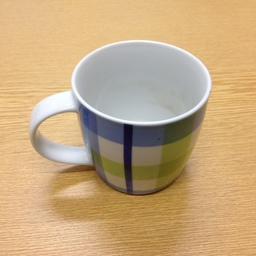
\includegraphics[width=.14\textwidth]{mug2} & 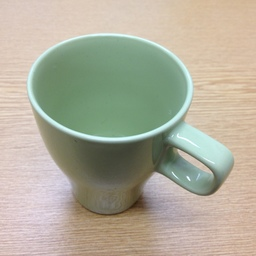
\includegraphics[width=.14\textwidth]{mug3} & 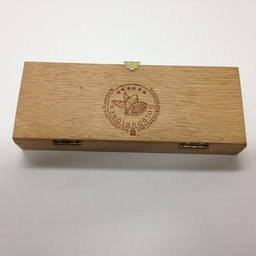
\includegraphics[width=.14\textwidth]{box1} & 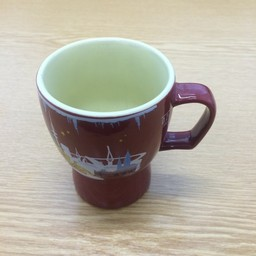
\includegraphics[width=.14\textwidth]{mug4} \\
        mug & mug & mug & not mug & mug \\
      \end{tabular}

  \end{itemize}
\end{frame}

\section{Feature Extraction}
\begin{frame}
  \frametitle{Bag-of-Words Model with SIFT Descriptors}

  \begin{itemize}
    \item SIFT Descriptor~\cite{lowe_object_1999}. 
      \begin{itemize}
        \item Local feature descriptor invariant to several image transforms.
        \item Standard for object recognition in robotics.

          ~
        \item Does not describe the whole image/object.
        \item Does not encode general features of a category.
      \end{itemize}
  \end{itemize}

  \centering
  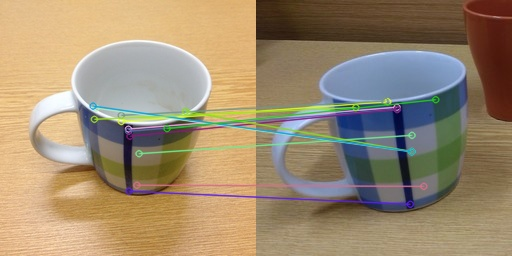
\includegraphics[width=.7\textwidth]{mug2m}
\end{frame}

\begin{frame}
  \frametitle{Bag-of-Words Model with SIFT Descriptors}

  \begin{itemize}
    \item Bag-of-words model~\cite{csurka_visual_2004}. 
      \begin{itemize}
        \item A document : a collection of words.
        \item Count occurrences and ignore order. 

          ~
        \item An image : a collection of local features.
        \item Vector quantization with codebook.
      \end{itemize}
      ~
  \end{itemize}
\end{frame}

\begin{frame}
  \frametitle{Mel-frequency Cepstrum Coefficients}

  \begin{itemize}
    \item DCT of log power spectrum at mel-scale.
    \item MFCCs are common features for audio processing, such as speech recognition and speaker recognition.
  \end{itemize}
\end{frame}

\section{Hidden Markov Models}
\begin{frame}
  \frametitle{Hidden Markov Models}

  \begin{itemize}
    \item HMM describes a distribution of a stochastic process~\cite{rabiner_fundamentals_1993}.
      \begin{itemize}
        \item Applications in speech recognition and gesture recognition. 
        \item Images and sound change over time during interaction.
      \end{itemize}
      ~

    \item HMM assumes there is a hidden state variable associated with the observation at each time.
      \begin{itemize}
        \item Observation sequence: \[ \mathbf{x} = x_1 x_2 \dots x_T . \]
        \item State sequence: \[ \mathbf{q} = q_1 q_2 \dots q_T . \]
      \end{itemize}
  \end{itemize}
\end{frame}

\begin{frame}
  \frametitle{Two Properties}

  \centering
  \includegraphics[width=.5\textwidth]{hmm.tikz}

  \begin{itemize}
    \item The present observation (at a certain time $t$) depends only upon the present hidden state:
      \[
        P(x_t|q_1, \dots, q_t, x_1, \dots, x_{t-1},x_{t+1},\dots,x_T) = P(x_t|q_t) .
      \]
    \item (Markov property) The future hidden state depends only upon the present state:
      \[
        P(q_{t+1}|q_1, \dots, q_t, x_1, \dots, x_t) = P(q_{t+1}|q_t) .
      \]
  \end{itemize}
\end{frame}

\begin{frame}
  \frametitle{Parameters of HMM}

  \begin{itemize}
    \item $ \lambda = (A, B, \pi) $
    \item Transition probability : $A = \{a_{ij}\}$, in which 
      \[ a_{ij} = P(q_{t+1} = j | q_t = i) \]
    \item Observation distribution, $B = \{b_j(x)\}$, in which
      \[ b_j(x) = P(x_t = x | q_t = j) \]
      PDF of GMM:
      \[ b_j(x) = \sum_{k=1}^M c_{jk} \mathcal{N}(x, \mu_{jk}, \Sigma_{jk}) \]
    \item Initial state distribution, $\pi = \{\pi_j\}$, in which
      \[ \pi_j = P(q_1 = j) \]
  \end{itemize}
\end{frame}

\begin{frame}
  \frametitle{Basic Problems of HMM}

  \begin{itemize}
    \item Probability evaluation: $ P(\mathbf{x}|\lambda) $.
      \begin{itemize}
        \item Forward/backward procedure. 
      \end{itemize}

    \item Most likely state sequences: $ \argmax_{\mathbf{q}} P(\mathbf{x}|\mathbf{q},\lambda) $.
      \begin{itemize}
        \item Viterbi algorithm.
      \end{itemize}

    \item Parameter estimation: $ \argmax_{\lambda} P(\mathbf{x}|\lambda) $.
      \begin{itemize}
        \item Baum-Welch Algorithm (EM Algorithm).
        \item Note: MLE is not assured.
      \end{itemize}
  \end{itemize}
\end{frame}

\begin{frame}
  \frametitle{Choices of HMM}

  \begin{itemize}
    \item \# of states, $N$: \hfill small <=> large.
    \item \# of mixture components $M$: \hfill small <=> large.
    \item Covariance matrix: \hfill diagonal <=> full.
  \end{itemize}
  ~
  \begin{columns}
    \begin{column}{.4\textwidth}
      \centering simple
    \end{column}
    \begin{column}{.2\textwidth}
      \centering <=>
    \end{column}
    \begin{column}{.4\textwidth}
      \centering complex
    \end{column}
  \end{columns}
  \begin{columns}
    \begin{column}{.5\textwidth}
      \begin{itemize}
        \item Smaller hypothesis space.
        \item Easy to learn.
        \item Biased result.
        \item Underfitting.
      \end{itemize}
    \end{column}
    \begin{column}{.5\textwidth}
      \begin{itemize}
        \item Larger hypothesis space.
        \item Hard to learn.
        \item More approximate result.
        \item Overfitting.
      \end{itemize}
    \end{column}
  \end{columns}
\end{frame}

\begin{frame}
  \frametitle{Classification with HMM}

  \begin{itemize}
    \item Estimate $\lambda^c$ with all data of class $c$.
    \item Approximate likelihood with learned model:
      \[ P(\mathbf{x}|c) = P(\mathbf{x}|\lambda^c) . \]
    \item Specific object recognition (multiclass classification):
      \[ f(\mathbf{x}) = \argmax_{c} P(\mathbf{x}|c) \]
    \item Generic category recognition (binary classification):
      \[ 
        f(\mathbf{x}) = \left\{
          \begin{array}{l l}
            +1, & \quad P(c=+1|\mathbf{x}) > \theta; \\
            -1, & \quad \text{otherwise.}
          \end{array} \right.
        \]
        where
        \[ P(c|\mathbf{x}) = \frac{P(\mathbf{x}|c)P(c)}{\sum_{c \in \{-1,+1\}} P(\mathbf{x}|c)P(c)} . \]
    \end{itemize}
  \end{frame}

  \section{Bimodal Object Recognition}
  \begin{frame}
    \frametitle{Multimodal Fusion Methods}

    \begin{itemize}
      \item $\mathbf{x} = (\mathbf{v},\mathbf{a})$.
      \item The goal is to compute the joint likelihood:
        \[ P(\mathbf{v},\mathbf{a}|c) \]

        ~
      \item Two approaches:
        \begin{itemize}
          \item Feature Fusion.
          \item Decision Fusion.
        \end{itemize}
    \end{itemize}
  \end{frame}

  \begin{frame}
    \frametitle{Feature Fusion}

    \centering
    \includegraphics{featurefs.tikz}

    \begin{itemize}
      \item Directly learn the joint likelihood with concatenated features:
        \[ P(\mathbf{v},\mathbf{a}|c) = P(\mathbf{v},\mathbf{a}|\lambda_{va}^c) \]
    \end{itemize}
  \end{frame}

  \begin{frame}
    \frametitle{Decision Fusion}

    \centering
    \includegraphics{decisionfs.tikz}

    \begin{itemize}
      \item Learn separate models and combine them under conditional independence assumption:
        \[ P(\mathbf{v},\mathbf{a}|c) = P(\mathbf{v}|c) P(\mathbf{a}|c) = P(\mathbf{v}|\lambda_v^c) P(\mathbf{a}|\lambda_a^c) \]
    \end{itemize}
  \end{frame}

  \section{Experiment}
  \begin{frame}
    \frametitle{Experiment Setup}

    \begin{itemize}
      \item 33 household objects.
    \end{itemize}

    \begin{columns}
      \begin{column}{.45\textwidth}
        \begin{itemize}
          \item Interactions:
            \begin{itemize}
              \item Knock with a stick.
              \item Push.
              \item Shake.
            \end{itemize}
        \end{itemize}
      \end{column}
      \begin{column}{.45\textwidth}
        \begin{itemize}
          \item Categories:
            \begin{itemize}
              \item Mugs.
              \item Bottles.
              \item Plastic objects.
              \item Metal objects.
              \item Fragile objects.
              \item Containers with content.
            \end{itemize}
        \end{itemize}
      \end{column}
    \end{columns}
  \end{frame}

  \begin{frame}
    \frametitle{Specific Object Recognition Result}

    \centering
    \begin{tabular}[h]{c|c}
      \hline
      Method & Accuracy \\ \hline \hline
      Feature Fusion & \underline{95.8\%} \\ \hline
      Decision Fusion  & 95.7\% \\ \hline
      Visual Only & 86.7\% \\ \hline
      Audio Only & 83.6\% \\ \hline
    \end{tabular}

    ~
    \begin{itemize}
      \item 5-fold cross validation.
      \item HMM with 2 states, 6 mixture components and diagonal covariance matrix.
    \end{itemize}
    \vfill
    {\scriptsize
      \[ \text{accuracy} =  \frac{\text{\# correctly classified}}{\text{\# total}} \]
    }
  \end{frame}

  \begin{frame}
    \frametitle{Generic Category Recognition Result}

    \begin{columns}
      \begin{column}{.5\textwidth}
        \centering
        \scriptsize
        \includegraphics[width=\columnwidth]{roc.tikz}
      \end{column}
      \begin{column}{.5\textwidth}
        \begin{itemize}
          \item Object-based cross validation.
          \item Receiver operating characteristic (ROC).
          \item Area under the curve (AUC).
            \begin{itemize}
              \item 0.5 => Random
              \item 1.0 => Perfect 
            \end{itemize}
        \end{itemize}
      \end{column}
    \end{columns}
    {\scriptsize
      \[ \text{true positive rate} =  \frac{\text{\# true positive}}{\text{\# conditional positive}} \]
      \[ \text{false positive rate} =  \frac{\text{\# false positive}}{\text{\# conditional negative}} \]
    }
  \end{frame}

  \begin{frame}
    \frametitle{Generic Category Recognition Result}

    \begin{columns}
      \begin{column}{.6\textwidth}
        \centering
        \footnotesize
        \includegraphics[width=\columnwidth]{mug.tikz}
      \end{column}
      \begin{column}{.4\textwidth}
        \begin{itemize}
          \item Mugs
        \end{itemize}
        ~

        \footnotesize
        \begin{tabular}[h]{c|c}
          \hline
          Method & AUC \\ \hline \hline
          Feature Fusion & 0.750 \\ \hline
          Decision Fusion  & \underline{0.771} \\ \hline
          Visual Only & 0.763 \\ \hline
          Audio Only & 0.642 \\ \hline
        \end{tabular}
      \end{column}
    \end{columns}
  \end{frame}

  \begin{frame}
    \frametitle{Generic Category Recognition Result}

    \begin{columns}
      \begin{column}{.6\textwidth}
        \centering
        \footnotesize
        \includegraphics[width=\columnwidth]{bottle.tikz}
      \end{column}
      \begin{column}{.4\textwidth}
        \begin{itemize}
          \item Bottles
        \end{itemize}
        ~

        \footnotesize
        \begin{tabular}[h]{c|c}
          \hline
          Method & AUC \\ \hline \hline
          Feature Fusion & \underline{0.802} \\ \hline
          Decision Fusion  & 0.798 \\ \hline
          Visual Only & 0.778 \\ \hline
          Audio Only & 0.707 \\ \hline
        \end{tabular}
      \end{column}
    \end{columns}
  \end{frame}

  \begin{frame}
    \frametitle{Generic Category Recognition Result}

    \begin{columns}
      \begin{column}{.6\textwidth}
        \centering
        \footnotesize
        \includegraphics[width=\columnwidth]{plastic.tikz}
      \end{column}
      \begin{column}{.4\textwidth}
        \begin{itemize}
          \item Plastic objects
        \end{itemize}
        ~

        \footnotesize
        \begin{tabular}[h]{c|c}
          \hline
          Method & AUC \\ \hline \hline
          Feature Fusion & 0.820 \\ \hline
          Decision Fusion & \underline{0.839} \\ \hline
          Visual Only & 0.813 \\ \hline
          Audio Only & 0.732 \\ \hline
        \end{tabular}
      \end{column}
    \end{columns}
  \end{frame}
  \begin{frame}
    \frametitle{Generic Category Recognition Result}

    \begin{columns}
      \begin{column}{.6\textwidth}
        \centering
        \footnotesize
        \includegraphics[width=\columnwidth]{metal.tikz}
      \end{column}
      \begin{column}{.4\textwidth}
        \begin{itemize}
          \item Metal objects
        \end{itemize}
        ~

        \footnotesize
        \begin{tabular}[h]{c|c}
          \hline
          Method & AUC \\ \hline \hline
          Feature Fusion & 0.830 \\ \hline
          Decision Fusion  & 0.870 \\ \hline
          Visual Only & \underline{0.877} \\ \hline
          Audio Only & 0.772 \\ \hline
        \end{tabular}
      \end{column}
    \end{columns}
  \end{frame}
  \begin{frame}
    \frametitle{Generic Category Recognition Result}

    \begin{columns}
      \begin{column}{.6\textwidth}
        \centering
        \footnotesize
        \includegraphics[width=\columnwidth]{fragile.tikz}
      \end{column}
      \begin{column}{.4\textwidth}
        \begin{itemize}
          \item Fragile objects
        \end{itemize}
        ~

        \footnotesize
        \begin{tabular}[h]{c|c}
          \hline
          Method & AUC \\ \hline \hline
          Feature Fusion & 0.711 \\ \hline
          Decision Fusion  & 0.697 \\ \hline
          Visual Only & 0.590 \\ \hline
          Audio Only & \underline{0.819} \\ \hline
        \end{tabular}
      \end{column}
    \end{columns}
  \end{frame}
  \begin{frame}
    \frametitle{Generic Category Recognition Result}

    \begin{columns}
      \begin{column}{.6\textwidth}
        \centering
        \footnotesize
        \includegraphics[width=\columnwidth]{nonempty.tikz}
      \end{column}
      \begin{column}{.4\textwidth}
        \begin{itemize}
          \item Containers with contents
        \end{itemize}
        ~

        \footnotesize
        \begin{tabular}[h]{c|c}
          \hline
          Method & AUC \\ \hline \hline
          Feature Fusion & 0.671 \\ \hline
          Decision Fusion  & \underline{0.675} \\ \hline
          Visual Only & 0.567 \\ \hline
          Audio Only & 0.620 \\ \hline
        \end{tabular}
      \end{column}
    \end{columns}
  \end{frame}

  \section{Conclusion}
  \begin{frame}
    \frametitle{Conclusion}

    \begin{itemize}
      \item For specific object recognition, both fusion methods increased the accuracy for about 10\%, comparing to unimodal methods.

        ~
      \item For generic category recognition, both fusion methods increased the performance under the condition of neither of the modality is noise.

        ~
      \item There is no significant difference in performance between the two fusion methods.
        \begin{itemize}
          \item Visual and audio signals are independent under the condition of being in one category.
          \item Visual and audio signals are congruent in our dataset.
        \end{itemize}
    \end{itemize}
  \end{frame}

  \begin{frame}
    \frametitle{Future Work}

    \begin{itemize}
      \item Real-time recognition.
        \begin{itemize}
          \item SIFT => SURF.
        \end{itemize}

      \item Increase dataset.
        \begin{itemize}
          \item Collect data by robots or from Internet sources.
          \item More data make it possible to use discriminant methods to learn combination rules.
        \end{itemize}

      \item Learn good features using multimodal signals.
        \begin{itemize}
          \item Congruency as a heuristic.
          \item Using deep learning neural networks~\cite{ngiam_multimodal_2011}.
        \end{itemize}
    \end{itemize}
  \end{frame}

  \frame[c]{
    \frametitle{The End}
    \begin{center}
      Thank you for your attention.\\[1ex]
      Any question?\\[5ex]
    \end{center}
  }

  \appendix
  \section*{References}
  \begin{frame}[allowframebreaks]
    \frametitle{References}
    {\scriptsize
      \bibliography{thesis}
      \bibliographystyle{unsrt}  
    }
  \end{frame}

  \end{document}

